
%(BEGIN_QUESTION)
% Copyright 2011, Tony R. Kuphaldt, released under the Creative Commons Attribution License (v 1.0)
% This means you may do almost anything with this work of mine, so long as you give me proper credit

Anta at følgende magnetventilstyrte ventilsystem fungerer som det skal under normal drift (dvs. ingen nødsituasjoner, ingen unormale forhold).  Trykket i prosesstanken er stabilt 75 PSI på trykkmåleren (PG), og den pneumatisk opererte ventilen PCV-5 er av typen ``air-to-open'':

$$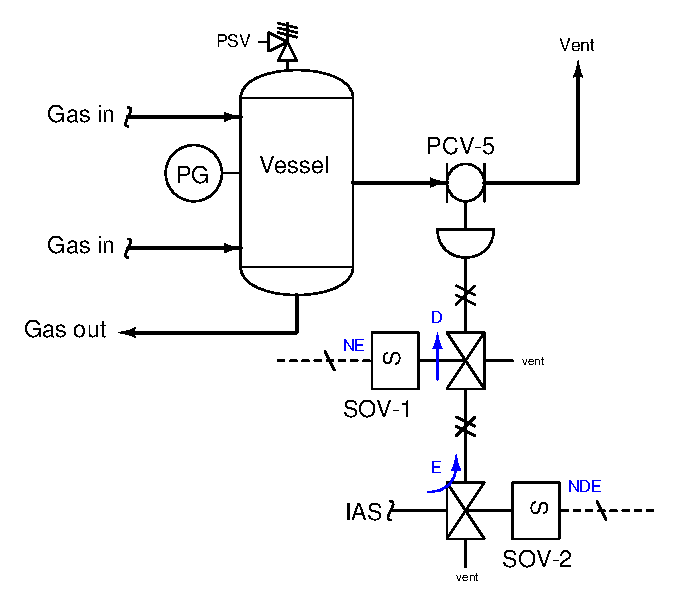
\includegraphics[width=15.5cm]{i00299x01.eps}$$

\noindent
Velg det beste svaret som beskriver umiddelbar effekt på prosessen hvis magnetventil SOV-2 plutselig får en ``åpen'' elektrisk feil i spolen:

\begin{itemize}
\item{} Tanken imploderer umiddelbart på grunn av raskt fall i internt gasstrykk
\vskip 10pt
\item{} Trykket i prosesstanken begynner å stige når PCV-5 stenger og fanger gass
\vskip 10pt
\item{} Trykket i prosesstanken begynner å falle når PCV-5 lufter gass til atmosfære
\vskip 10pt
\item{} Prosessen fortsetter normal drift og holder 75 PSI i tanken
\end{itemize}

\underbar{file i00299}
%(END_QUESTION)





%(BEGIN_ANSWER)

Prosessen fortsetter normal drift og holder 75 PSI i tanken.

%(END_ANSWER)





%(BEGIN_NOTES)

{\bf This question is intended for exams only and not worksheets!}.

%(END_NOTES)
